\documentclass[11pt]{beamer}
% Packages
\usepackage{beamer-german}


% Title etc.
\title{Authoritarian Notions of Democracy}
\subtitle{Analyse politischer Unterstützung in der quantitativen Forschungspraxis}
\date{04. Februar 2022}
\author{B. Philipp Kleer}
\institute{Institut für Politikwissenschaft | Justus-Liebig-Universität Gießen}

\setbeamerfont{itemize/enumerate body}{size = \small}
\setbeamerfont{itemize/enumerate subbody}{size = \footnotesize}
\setbeamerfont{itemize/enumerate subsubbody}{size = \scriptsize}

% Datumspaket
\usepackage[german]{isodate}

% Table packages
\usepackage{booktabs}
\usepackage{longtable}

\addbibresource{lit-s11.bib}

\begin{document}

\begin{frame}
	\maketitle
\end{frame}


\begin{frame}[t]{Ansätze zum Messen autoritärer Werteorientierungen}
 Wie wurden bisher antidemokratische Werteorientierungen/Einstellungen empirisch operationalisiert?
 
	\begin{abclist}
	 	\item Unterstützung Systemalternativen
	 	\item Emanzipatorische Werte
	 	\item autoritäre Orientierungen
	 	\item Ansatz verschiedener Demokratieverständnisse
	\end{abclist}
\end{frame}

\begin{frame}{Unterstützung Systemalternativen}
Anti-demokratische Tendenzen gemessen über \shine{Zustimmung zu Systemalternativen}:

	\begin{itemize}
		\item oftmals in der Transformationsforschung genutzt (vgl. \parencite{Linz1996, Rose1998})
		\item aus Negation der alternativen Systemformen (Militärregierung, einzelne:r Führer:in, Expertenregierung) wird in Kombination mit Unterstützung des demokratischen Systems auf demokratische Einstellung geschlossen
	\end{itemize}

\end{frame}

\begin{frame}{Unterstützung Systemalternativen}
\shine{Our current system of government is not the only one that this country has had. Some people say that we would be better off if the country was governed differently. What do you think?}
	\begin{itemize}
		\item Return to communist rule
		\item Army should govern
		\item Strong leader without parliament
		\item Return to monarchy
		\item Economy should be run by experts \parencite[111]{Rose1998}
	\end{itemize}
\end{frame}

\begin{frame}{Unterstützung Systemalternativen}
\shine{Which of the following statements do you agree with most?}
	\begin{nolist}
		\item Democracy is preferable to any other kind of government
		\item In certain situations an authoritarian government can be preferable to a democratic one
		\item To people like me, it doesn't matter whether we have a democratic government or a non-democratic governemt \parencite[103]{Rose1998}
	\end{nolist}
\end{frame}

\begin{frame}{Index emanzipatorischer Werte \parencite[71]{Welzel2013}}
	\begin{figure}[ht]
		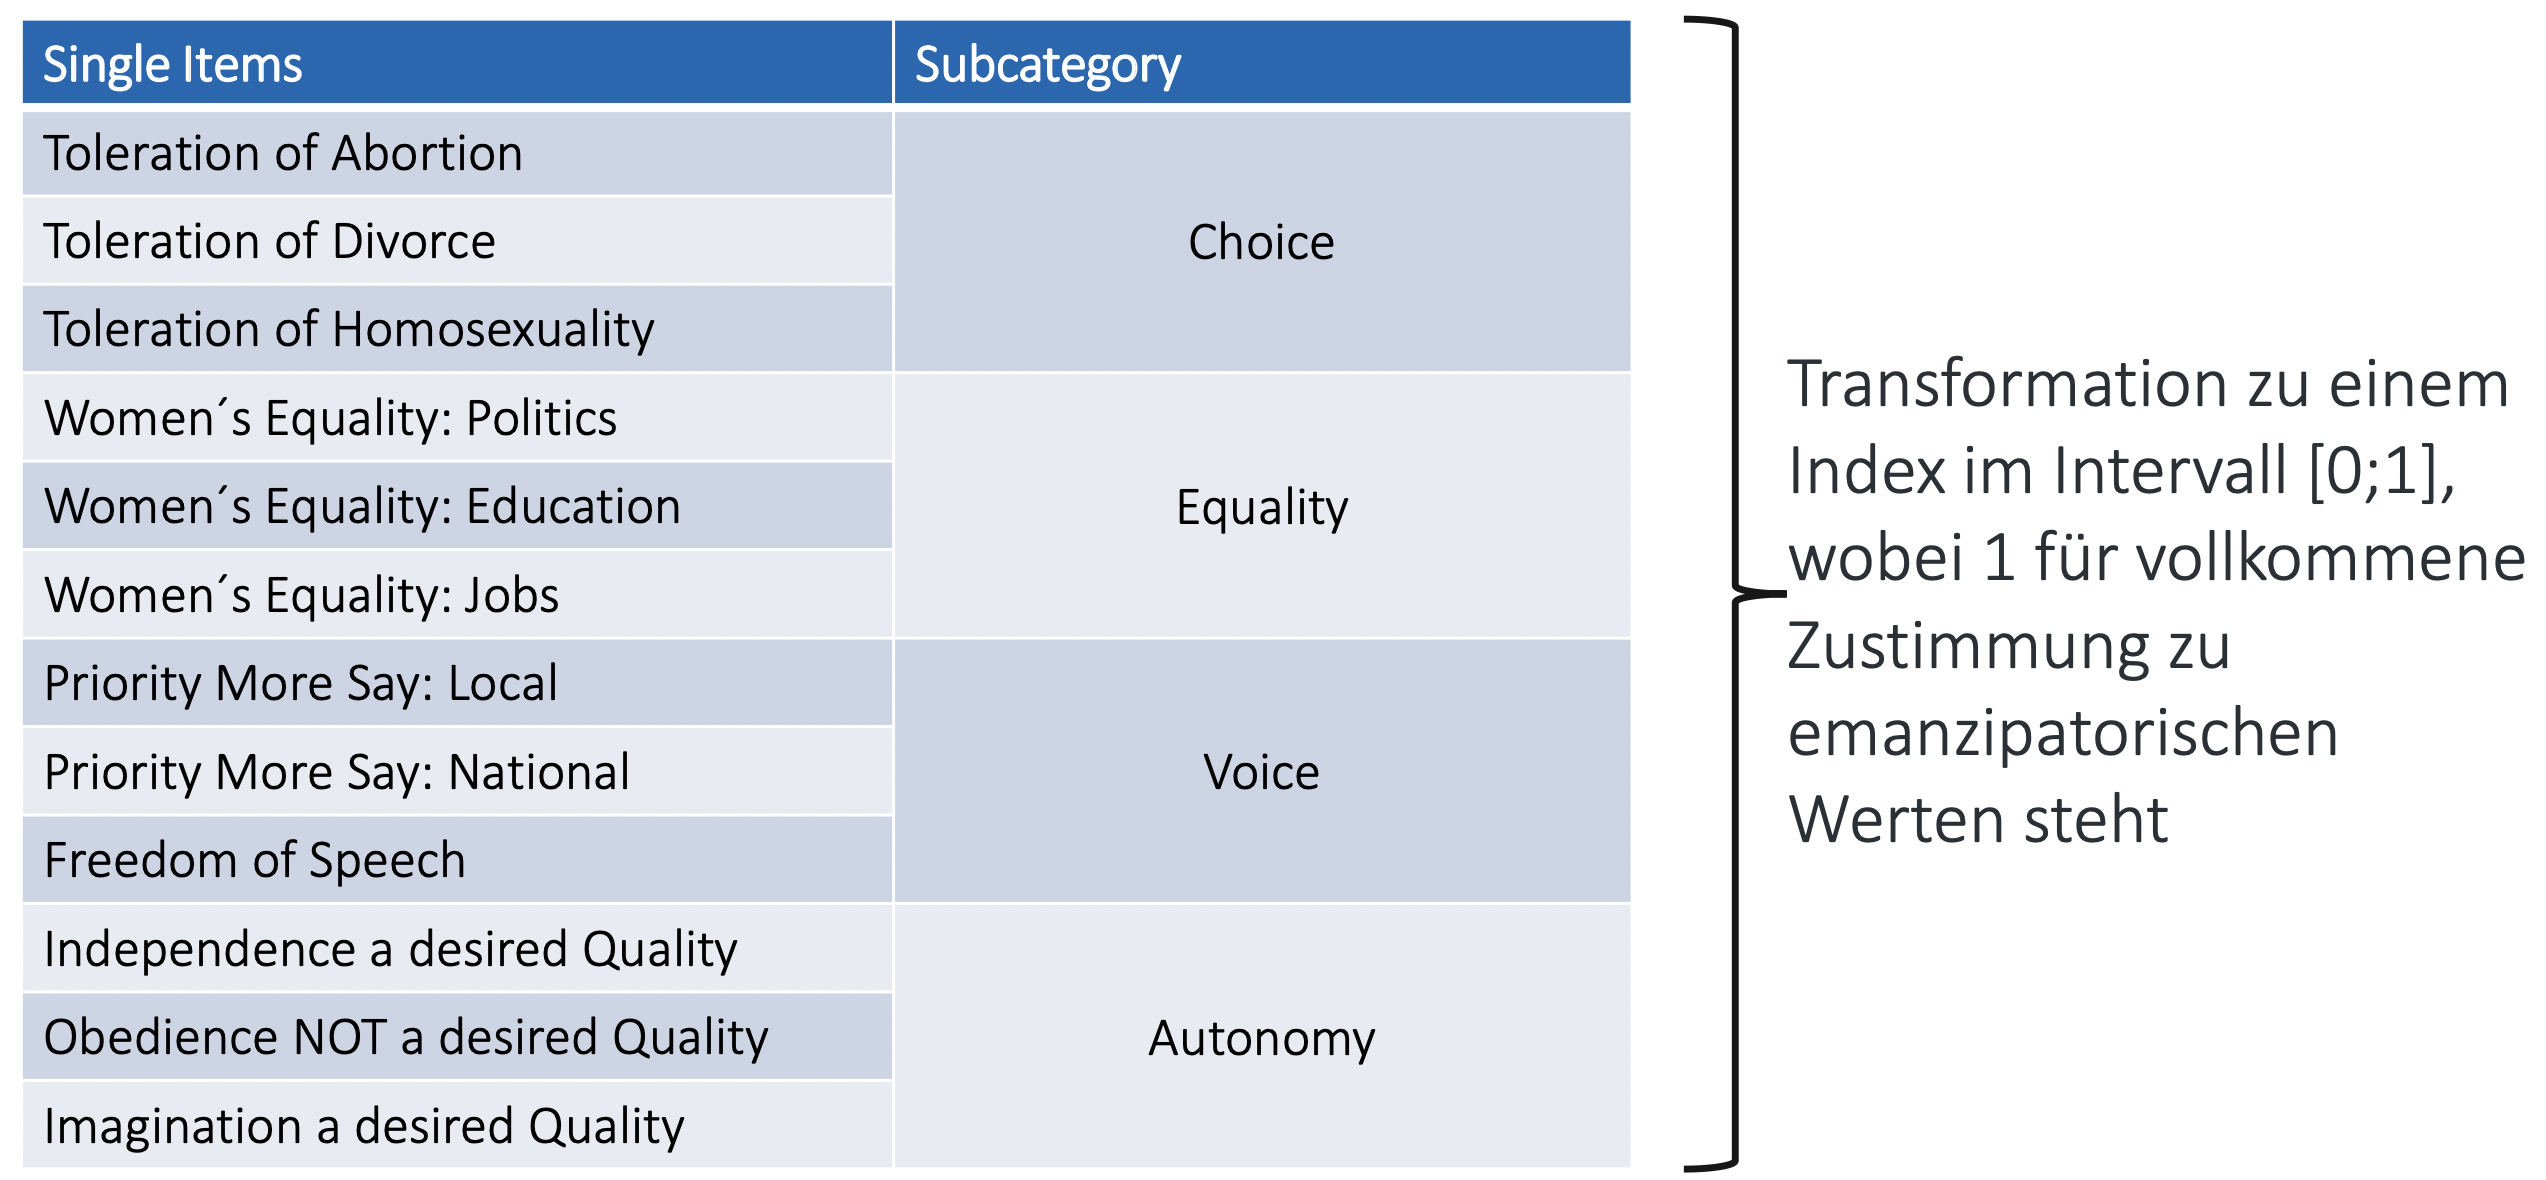
\includegraphics[width=\textwidth]{pics/s11-1.png}
		\caption{\textbf{Itemliste}}
	\end{figure}
\end{frame}

\begin{frame}{Index emanzipatorischer Werte \parencite[71]{Welzel2013}}
	\begin{itemize}
		\item Antidemokratische Werteorientierungen würden kompatibel mit diesem Ansatz ausdrücken, dass es sich um das Nicht-Vorhandensein emanzipatorischer Werte handelt.
		\item empirisch bedeuten würde dies heißen, dass es eine Abkehr von der Unterstützung individueller Freiheiten geben muss.
		\begin{itemize}
			\item denkbar: Schutz von Minderheitenrechten, Selbstbestimmungsrechte von Frauen
		\end{itemize}
		\item \cite[399]{Welzel2007}: emanzipatorische Werteorientierungen sind bei einem bereits hohen Level von Demokratie ein Unterstützungsfaktor, der die Demokratie „stabilisert“.
	\end{itemize}
\end{frame}

\begin{frame}{Autoritäre Orientierungen}
	\begin{itemize}
		\item \cite{Spier2010} misst autoritäre Werteorientierung über Items der Schwartz-Batterie identifiziert drei relevante Items aus Schwartz-Batterie für Autoritarismus
		\begin{itemize}
			\item Es ist ihm/ihr wichtig, sich jederzeit korrekt zu verhalten. Er/Sie vermeidet es, Dinge zu tun, die andere Leute für falsch halten könnten.
			\item Er/Sie glaubt, dass die Menschen tun sollten, was man ihnen sagt. Er/Sie denkt, dass Menschen sich immer an Regeln halten sollten, selbst dann, wenn es niemand sieht.
			\item Es ist ihm/ihr wichtig, dass der Staat seine/ihre persönliche Sicherheit vor allen Bedrohungen gewährleistet. Er/Sie will einen starken Staat, der seine Bürger verteidigt
		\end{itemize}
	\end{itemize}
\end{frame}

\begin{frame}{Verschiedene Demokratiemodelle}
	\begin{itemize}
		\item Ausgangspunkt: Demokratiekritik/-unzufriedenheit beruht auf verschiedener Definition von Demokratie
		\item Identifizierung von 4 Demokratiemodellen:
		\begin{itemize}
			\item Trustee Model of Democracy,
			\item Anti-pluralist scepticism,
			\item Deliberative proceduralism,
			\item Populist majoritarianism \parencite[792]{Landwehr2017}
		\end{itemize}
	\end{itemize}
\end{frame}

\begin{frame}{Typen Demokratiemodelle I} 
	\begin{table}[ht]
		\tiny
		\begin{tabular}{>{\raggedright}m{0.6\textwidth} >{\centering\arraybackslash}m{0.3\textwidth} }
			\toprule[2pt]
			Item & Konzept \\
			\midrule
			The government should stick to planned policies even if a majority of cititzens is against them. & \multirow{4}{*}{Trustee model of democracy} \\
			Sometimes it is better when political decisions are taken behind closed doors. &  \\
			Members of parliament should follow their conscience even if a majority of citizens happens to hold different opinions. & \\
			The government should change planned policies if a majority of citizens no longer supports them. & \\
			\midrule
			Struggles between different interest groups in our society damage the common good. & \multirow{5}{*}{Anti-pluralist scepticism} \\
			It would be better if important political decisions were taken by independent experts rather than elected politicians. & \\
			Important political decisions should be taken only with approval of all affected groups. & \\
			Important political decisions should be taken in deliberation and not through mere voting. &\\
			In general, conflicts cannot be resolved through discussion and negotiation. & \\			
			\bottomrule[2pt]
		\end{tabular}
		\caption{\cite{Landwehr2017}}
	\end{table}
\end{frame}

\begin{frame}{Typen Demokratiemodelle II} 
	\begin{table}[ht]
		\tiny
		\begin{tabular}{>{\raggedright}m{0.6\textwidth} >{\centering\arraybackslash}m{0.3\textwidth} }
			\toprule[2pt]
			Item & Konzept \\
			\midrule
			One has to accept democratically taken decisions in any case, even if they conflict with own interests. & \multirow{4}{*}{Deliberative proceduralism} \\
			In political decisions, the common good and not the own interest should be the central focus. &  \\
			It is important in democracy to understand why other people have different opinions. & \\
			The government should develop policies in close dialogue with citizens and affected groups. & \\
			\midrule
			Minority rights must be protected from majority decisions. & \multirow{3}{*}{Populist majoritarianism} \\
			Majority decisions must apply, even if they curtail minority rights. & \\
			If there is a large majority in the population for a political decisions, this indicates that the decision is correct. & \\
			\bottomrule[2pt]
		\end{tabular}
		\caption{\cite{Landwehr2017}}
	\end{table}
\end{frame}

\begin{frame}{Authoritarian Notions of Democracy}
	\begin{itemize}
		\item Paradox of Democracy: "widespread support for democracy often coexists with severe deficiencies in the latter, including its outright absence” \parencite[307]{Welzel2013}
		\item liberal notions of democracy (\shine{LND}) vs. authoritarian notions of democracy (\shine{AND})
		\item Unterstützung emanzipatorischer Werte dagegen kann Zustand der Demokratie besser erklären als Unterstützung der Demokratie
		\item Emanzipatorische Werte erklären sowohl individuelle \shine{AND} als auch \shine{AND} auf Makroebene
		\item je höher \shine{AND} in einem Land, desto mehr überschätzen Personen in dem Land den "demokratischen Status”
	\end{itemize}

\end{frame}

\begin{frame}{LND \& AND}
	\begin{figure}[ht]
		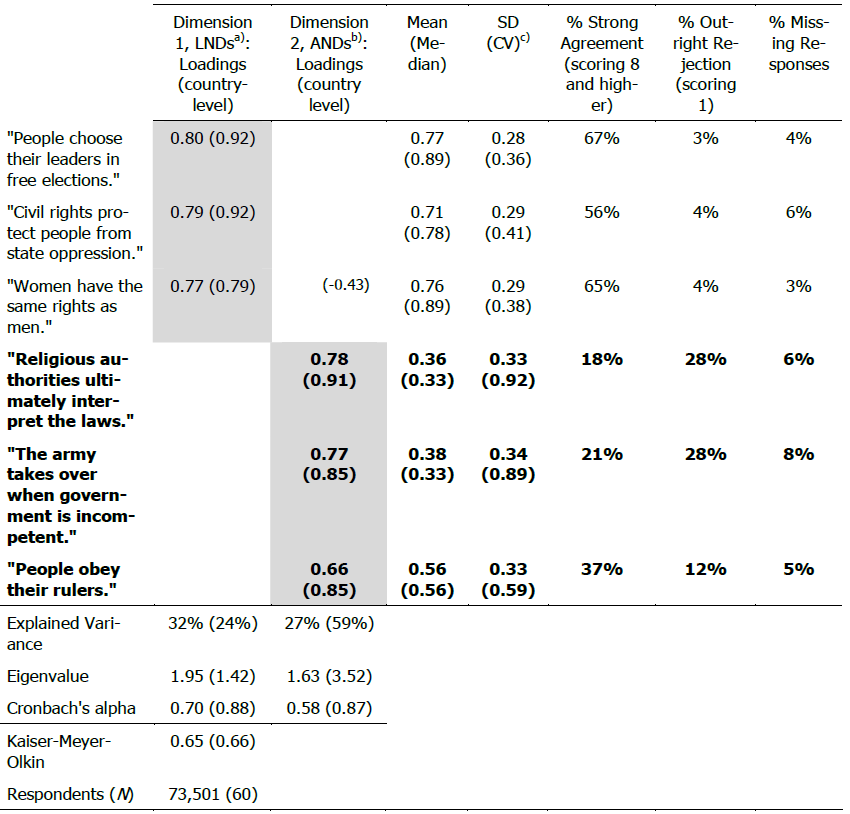
\includegraphics[width=.8\textwidth]{pics/s11-2.png}
		\caption{\textbf{\cite[7]{Welzel2017}}}
		\label{Fig:XXX}
	\end{figure}
\end{frame}

\begin{frame}{Multi-Level-Modelle}
	\begin{figure}[ht]
		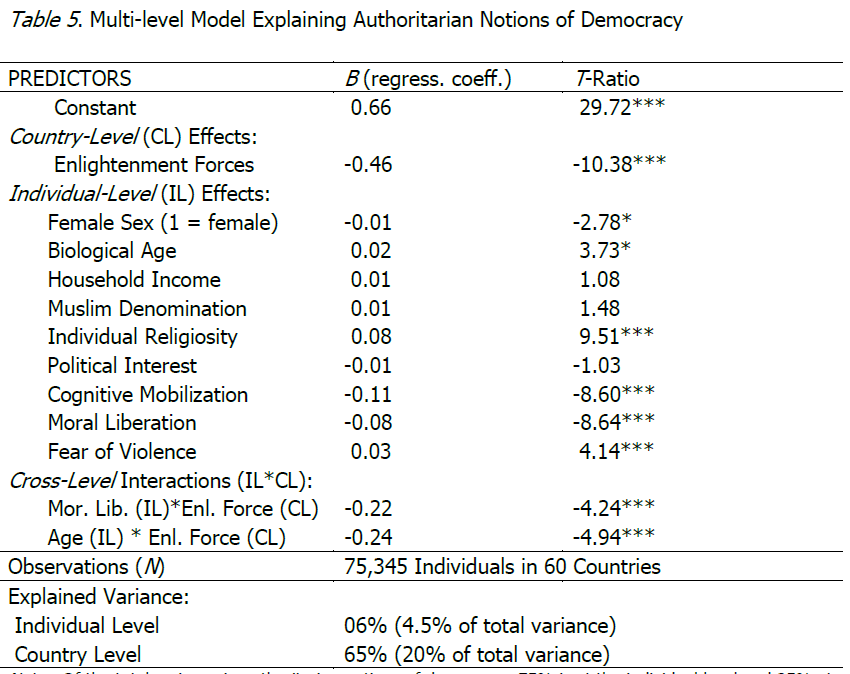
\includegraphics[width=.9\textwidth]{pics/s11-3.png}
		\caption{\textbf{\cite[22]{Welzel2017}}}
		\label{Fig:XXX}
	\end{figure}
\end{frame}

\begin{frame}{Praxisaufgabe}
Im World Values Survey ist der Index emanzipatorischer Werte direkt inkludiert (\shine{RESEMAVAL}). Ebenso sind im Datensatz mehrere Makro-Variablen der Weltbank, der UN und des V-Dem Projekts inkludiert (Ende des Datensatzes).

	\begin{nolist}
		\item Versucht den Index \shine{LND} oder \shine{AND} nachzubilden. 
		\item Vergleicht anhand zweier Variablen (in denen Gruppen gebildet sind), inwieweit die Gruppen dieser zwei Variablen sich im Wert der \shine{LND} und \shine{AND} Werte unterscheiden. 
		\item Wähle zwei bis vier Länder und vergleiche hier den Wert von \shine{LND} und \shine{AND} Werte. 
	\end{nolist}
\end{frame}

\renewcommand*{\bibfont}{\scriptsize}

\begin{frame}[allowframebreaks]{Literatur}
	\nocite{*}
	\printbibliography[heading = none]
\end{frame}



\section{Mittagspause! \\ Wir treffen uns um 12:30 Uhr wieder.}

\end{document}
